\section{Historical: Training-Recipe Checks and Noise-Input Sensitivity}
\label{sec:training-updates}

The original 188-parameter estimator remains the proposed method. The
checks below change its training recipe or select between two frozen
models; they do not add a new estimator architecture. Each study has its
own fresh test cases. Their numerical averages must not be pooled as if
they came from one experiment. A severe error means per-case channel
NMSE $>1$, not a measured communication outage or numerical divergence.

\subsection{All-Pilot Rician Training}

The original loss estimates a channel from 21 pilot columns and predicts
nine held-out columns. Inference uses all 30 columns. To test this change
in input geometry, we also trained using all pilot columns, following
the re-corruption principle~\cite{pang2021r2r}. For an observed magnitude
$z=|\mu+w|$, with noiseless mean $\mu=(GS+B)_{np}$ and
$w\sim\CN(0,v)$, draw an independent
$\eta\sim\CN(0,v)$ and fix $\alpha>0$. Form
\begin{equation}
 z_{\rm in}=|z+\alpha\eta|,\qquad
 z_{\rm target}=|z-\eta/\alpha|.
\end{equation}
The input and target complex-noise variances are
$v(1+\alpha^2)$ and $v(1+\alpha^{-2})$, respectively. The EM update uses
the first variance, and the predictive Rician loss uses the second.

This construction does not require the unobserved complex field. To
check its distribution, write $Y=\mu+w$ and rotate $\eta$ by $\arg Y$.
Circular symmetry leaves the rotated noise independent of $Y$ and
unchanged in distribution. The resulting complex noises are
$w+\alpha\eta'$ and $w-\eta'/\alpha$. They are jointly proper Gaussian,
with cross-covariance $v-v=0$. Their magnitudes are therefore independent
conditional on $\mu$. They are \emph{not} independent conditional on a
fixed saved magnitude $z$. Repeated artificial corruptions of one block
are augmentations, not new channels. This argument assumes known,
independent circular Gaussian field noise and fixed $\alpha$; it is not
an unbiased-channel-NMSE result. The predictive likelihood and channel
error remain different objectives.

An initial development screen used 2,304 training blocks, 384 validation
blocks, two initialization seeds (10401 and 10402), and ten epochs. Its
six primary cells had SNR $-5,5,15$ dB, RSR $5,12$ dB, and random
3--7 paths per user. The 384 primary test worlds and 128 separate stress
worlds were generated after model freezing. Fixed-final-epoch scores
were primary: original, $\alpha=0.5$, and $\alpha=1$ gave
$-12.392$, $-12.835$, and $-13.365$ dB, with severe rates
$1.562\%$, $0.521\%$, and $0.391\%$. The two seed gains for
$\alpha=0.5$ were $-0.222$ and $1.109$ dB; for $\alpha=1$ they were
$0.747$ and $1.198$ dB. Thus the screen supported testing $\alpha=1$,
not a universal gain or reduced failure rate. Checkpoints selected by
the common 21/9 validation loss were secondary in this small screen.

\subsection{Matched Full-Budget Comparison}

The larger study fixed $\alpha=1$ before generating new test data. It
used the original 16,384 training blocks and 2,048 validation blocks,
three matched initialization seeds (9101--9103), 20 epochs, Adam with
step size $10^{-3}$, and batches of 32. Both learned recipes retained the same
188 parameters and ten EM/filtering stages. New artificial noise was
drawn each epoch. Initialization and epoch data orders matched the
original runs. Matching examples and optimizer updates does not match
training operations, noise distributions, or objectives. The experiment
tests the whole training recipe, not pilot geometry alone; 20 epochs
do not establish convergence.

Both methods' primary checkpoints minimize equal-condition 21/9
validation Rician loss, with epoch zero eligible. This preserves the
original selection rule but may favor its training recipe. Final-epoch
comparisons are reported separately. The full-budget study contains
8,192 fresh worlds in two banks (seeds 20261014211001 and
20261014221001), with 32 cases per cell and bank. Its 126 primary
conditions cross SNR $-10$ to $20$ dB in 5 dB steps, RSR $5,12,20$ dB,
and random 3--7 or fixed $2,4,8,12,16$ paths per user. Here
$N=32$, $K=3$, and $P=30$. Two stress cells add 128 worlds but do not
enter the primary metric. Offline and per-block rank-selected OptShrink
reuse frozen validation choices; per-block selection scores ranks
0--15 on 21/9 columns and refits all 30 columns.

The primary score pools the two banks' squared errors and channel powers
within each cell, takes their dB ratio, averages the 126 cells equally,
then averages the three model-specific scores. This is neither an
ensemble nor the dB of one pooled full-range ratio. All-pilot training
improves this score by $0.277$ dB over the original, but is $0.171$ dB
worse than block-rank OptShrink. It wins 106/126 cells against the
original, with a largest observed loss of $0.527$ dB. Severe errors
increase from $2.819\%$ to $4.473\%$; hence the average improvement is
not a general reliability improvement. The final-epoch gain is
$0.242$ dB. All-pilot training reduces the nearly noiseless error floor
but remains far behind OptShrink there, and does not fix weak-reference
performance. Tables~\ref{tab:training-full}--\ref{tab:training-seeds}
give the sensitivity, uncertainty and training records.

The two declared average-gain intervals use 4,000 paired resamples
within bank/cell, with Bonferroni adjustment. Pairing is retained across
methods and model seeds. The intervals condition on the fitted models
and shared training dataset; three initializations are not three
independent training populations. CPU timings use one PyTorch thread,
float64, batch one, and three randomized repeats per condition. They
include initialization and rank search/refitting, but exclude loading,
file access, and offline fitting. Original and all-pilot inference take
about 4.81 ms, compared with 15.66 ms for offline OptShrink and
108.08 ms for block-rank OptShrink. These are measured implementation
costs, not a hardware-independent complexity claim.

\begin{figure*}[!t]
\centering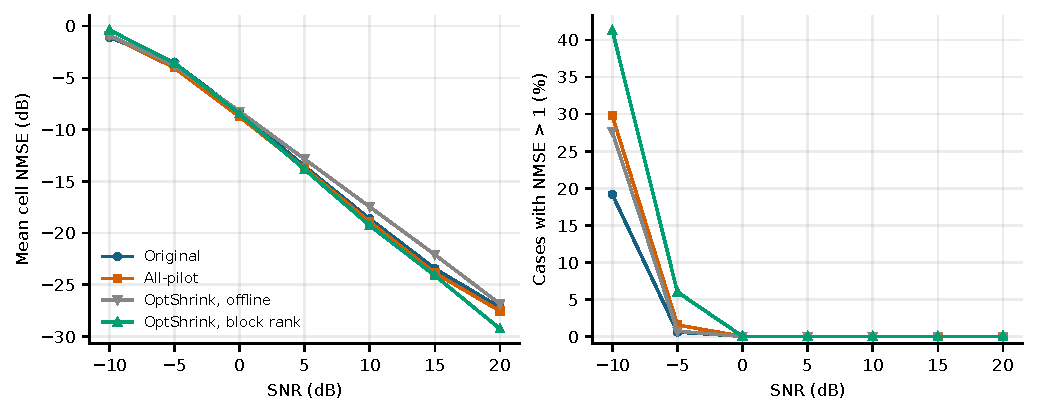
\includegraphics[width=\textwidth]{training_tradeoff.pdf}
\caption{The separate full-budget training comparison. Each SNR averages 18 reference/path conditions. Better average channel accuracy does not imply fewer severe errors. Curves use the same 8,064 primary worlds; neural scores average three fits, not an ensemble.}
\label{fig:training-tradeoff}
\end{figure*}

\subsection{One-Seed Mixed-Training Screen}

A separate test used seed 9101 and the same full training budget, with
exactly half the 512 batches per epoch assigned to each recipe. Each
batch still used one model evaluation and one optimizer update. The
two losses were averaged per measurement and logged separately; their
different noise levels make their raw scales incomparable. The same
21/9 validation rule selected epoch 19. Testing used 4,096 new worlds
(bank 20261015111001), including 4,032 primary and 64 stress worlds.

Mixed training improved the selected original by $0.152$ dB. Its
$0.033$ dB deficit to selected all-pilot training is descriptive: the
adjusted gain interval $[-0.0668,0.0008]$ dB includes zero. Its severe rate was
$3.745\%$, between the original's $2.902\%$ and all-pilot's $4.762\%$.
Compared with all-pilot, it corrected 42 severe outcomes and introduced
one; compared with the original, it introduced 34 and corrected none.
At $-10$ dB it reduced both mean-case error and severe frequency versus
all-pilot. At $-5$ dB it reduced severe frequency but increased mean-case
NMSE by $0.0100$. Its 5.008 ms runtime was only $0.56\%$ above the
original's measured time. Table~\ref{tab:training-mixed} retains all
selected/final results and the matched classical controls.

The predefined screen required a $0.2$ dB gain over the original,
lower mean-case error and severe frequency than all-pilot at both
$-10$ and $-5$ dB, an overall severe-rate increase of at most 0.2
percentage points over the original, and runtime at most $1.05$ times
the original. It passed the severe-frequency and runtime checks, but
failed the gain, low-SNR mean-error, and overall severe-rate checks.
This one-seed development result is not promoted to the main method.
Its 2,000 paired resamples condition on that one fit; only the four
macro-gain contrasts receive multiplicity adjustment. The screening
tolerances are practical rules, not statistical noninferiority claims.

\subsection{Simple Selection and Incorrect Noise Inputs}

We next froze the seed-9101 original and all-pilot models without
retraining. A scalar rule uses nominal SNR $10\log_{10}(3/\widetilde v)$
and selects the original below a threshold and all-pilot above it.
The constant 3 is the known expected signal power under this normalized
three-user benchmark, not the unknown realized channel power. The rule
is not established for arbitrary unknown path loss. Candidate cutoffs
were $-7.5,-2.5,2.5,7.5,12.5,17.5$ dB, plus both constant policies.
Selection used only the 2,048 validation observations, fixed 21/9
prediction loss, and equal condition weights, without channel labels.

Validation selected \emph{always original}: average loss 3.372665,
compared with 3.372740 for the 17.5 dB cutoff and 3.386371 for always
all-pilot. We did not force a switch or revise the cutoff after testing.
The 21/9 criterion may favor the original recipe and need not rank
all-30-pilot channel accuracy identically. This negative result rejects
this particular selection procedure, not every possible selector.

The new bank (20261015151001) has 4,224 worlds: 4,032 primary cases,
64 weak-reference/nearly-noiseless stress cases, and 128 off-grid cases
at SNR $\pm2.5$ dB with RSR 5/12 dB. Each physical observation is reused
with supplied variance $\widetilde v=v10^{\delta/10}$,
$\delta\in\{0,-3,+3\}$ dB. Raw magnitudes, pilots, reference, actual
noise, and true channels remain fixed. Every comparator and the router
receive the same biased variance. The three settings therefore are not
three independent test populations.

Table~\ref{tab:training-noise} shows a substantial sensitivity to noise
underestimation. The original's severe rate rises from $2.803\%$ with
correct variance to $11.111\%$ at $-3$ dB; the all-pilot rate rises
from $4.861\%$ to $14.509\%$. Overestimation by 3 dB gives $3.398\%$
and $5.432\%$, respectively. Because the frozen policy is constant,
there are no route changes and its estimates equal the original's.
The correct-noise $0.1$ dB gain criterion fails, although the severe-rate,
low-SNR and $1.05$ runtime criteria pass. The selector stores 376 model
weights plus the cutoff, evaluates only one 188-parameter model per
case, and takes 4.945 ms versus 4.875 ms for the original. No OptShrink
rerun is included in this screen. Its 2,000 paired intervals are
descriptive, conditional on the two fitted models, and unadjusted.

\subsection{Oracle Phase Diagnostic and Audit Scope}

A separate diagnostic uses 576 new worlds (seed 20261014031001), with
64 per SNR/RSR cell. It evaluates the three frozen original models at
SNR $-5,5,15$ dB and RSR $0,5,12$ dB. The raw, truth-aligned global-phase,
and truth-aligned antenna-row-phase average scores are $-10.833$,
$-10.912$, and $-12.853$ dB. The much larger row-wise change at weak
reference identifies an error component, not an implementable receiver
gain. Alignment can remove noise as well as phase error; it does not
prove a distinct local minimum or a physical reference-drift mechanism.
No learned setting is chosen from this diagnostic.

Saved audits checked paired identifiers, source/data/model hashes,
complete histories, frozen validation choices, finite outputs, and
representative prediction replays. The full-budget study replayed
384 neural and 64 independent classical predictions; mixed training
replayed 60 neural and 20 classical predictions; the selector replayed
1,188 predictions. Maximum neural discrepancies were below
$5\times10^{-15}$. This is not a replay of every training update.
The manuscript material generator independently recomputes primary
NMSE and severe rates from the saved error arrays. Small evidence files
retain all condition-level summaries, protocols, phase diagnostics,
selection scores and input hashes. These checks establish consistency
of the numerical record, not hardware validation, optimality,
convergence, or robustness to new training populations.

\begin{table*}[!t]
\caption{Full-budget study: selected and final-epoch sensitivity, plus separate stress cells. Primary scores use 8,064 worlds; each stress cell has 64 worlds. Weak reference: SNR 5/RSR 0 dB. Nearly noiseless: SNR 60/RSR 12 dB. Stress scores do not enter the primary score.}
\label{tab:training-full}\centering\footnotesize
\setlength{\tabcolsep}{3pt}
\begin{tabular}{@{}lrrrrr@{}}\toprule
Method & Macro (dB) & Pooled (dB) & Severe (\%) & Weak reference & Nearly noiseless\\
\midrule
Original (selected) & -13.684 & -6.650 & 2.82 & -7.244 & -6.949\\
All-pilot (selected) & -13.962 & -6.711 & 4.47 & -6.903 & -15.240\\
Original (final) & -13.762 & -6.684 & 3.04 & -7.280 & -6.921\\
All-pilot (final) & -14.005 & -6.695 & 4.61 & -6.865 & -23.116\\
OptShrink, block rank & -14.132 & -6.201 & 6.76 & -11.257 & -69.517\\
OptShrink, offline & -13.168 & -6.568 & 4.04 & -11.866 & -66.684\\
\bottomrule
\end{tabular}
\end{table*}

\begin{table*}[!t]
\caption{All-pilot gains: positive favors all-pilot training. Two predeclared contrasts, Bonferroni-adjusted conditional 95\% intervals. Worst observed harm is not a confidence bound.}
\label{tab:training-contrasts}\centering\footnotesize
\setlength{\tabcolsep}{3pt}
\begin{tabular}{@{}lrrrr@{}}\toprule
Comparator & Gain (dB) & 95\% interval & Cell wins & Worst harm\\
\midrule
Original (selected) & +0.277 & [+0.263, +0.294] & 106/126 & 0.527\\
OptShrink, block rank & -0.171 & [-0.221, -0.117] & 72/126 & 3.744\\
\bottomrule
\end{tabular}
\end{table*}

\begin{table}[!t]
\caption{Full-budget training records. Seeds share one training dataset. All-pilot training times include validation and concurrent-worker contention; they are not isolated-device benchmarks.}
\label{tab:training-seeds}\centering\footnotesize
\setlength{\tabcolsep}{3pt}
\begin{tabular}{@{}rrrrr@{}}\toprule
Seed & Original & All-pilot & Best epoch & Minutes\\
\midrule
9101 & -13.786 & -13.978 & 16 & 29.05\\
9102 & -13.446 & -13.938 & 18 & 28.99\\
9103 & -13.822 & -13.969 & 17 & 29.31\\
\bottomrule
\end{tabular}
\end{table}

\begin{table*}[!t]
\caption{Separate one-seed mixed-training screen: 4,032 primary worlds, not the full-budget test bank. Mean-case NMSE is linear. Selected-checkpoint comparisons are primary; final checkpoints are sensitivity checks.}
\label{tab:training-mixed}\centering\footnotesize
\setlength{\tabcolsep}{3pt}
\begin{tabular}{@{}lrrrr@{}}\toprule
Method & Macro (dB) & Case mean & Severe (\%) & Time (ms)\\
\midrule
Original (selected) & -13.799 & 0.2222 & 2.90 & 4.98\\
All-pilot (selected) & -13.984 & 0.2200 & 4.76 & 4.96\\
Mixed (selected) & -13.951 & 0.2163 & 3.75 & 5.01\\
Original (final) & -13.672 & 0.2224 & 3.00 & 4.98\\
All-pilot (final) & -14.004 & 0.2209 & 4.96 & 4.96\\
Mixed (final) & -13.966 & 0.2160 & 3.84 & 5.01\\
OptShrink, offline & -13.119 & 0.2257 & 4.69 & 16.06\\
OptShrink, block rank & -14.147 & 0.2454 & 6.70 & 115.20\\
\bottomrule
\end{tabular}
\end{table*}

\begin{table*}[!t]
\caption{Separate one-seed selector/noise-input screen: the same 4,032 primary worlds at all three supplied-variance offsets. Physical observations and actual noise are unchanged. The selected rule always runs the original model.}
\label{tab:training-noise}\centering\footnotesize
\setlength{\tabcolsep}{3pt}
\begin{tabular}{@{}rlrrrr@{}}\toprule
Offset (dB) & Method & Macro (dB) & Case mean & Severe (\%) & Time (ms)\\
\midrule
+0 & Original (selected) & -13.817 & 0.2228 & 2.80 & 4.88\\
+0 & All-pilot (selected) & -14.033 & 0.2207 & 4.86 & 4.86\\
+0 & Selected rule & -13.817 & 0.2228 & 2.80 & 4.95\\
-3 & Original (selected) & -13.195 & 0.4064 & 11.11 & 4.85\\
-3 & All-pilot (selected) & -13.007 & 0.4962 & 14.51 & 4.85\\
-3 & Selected rule & -13.195 & 0.4064 & 11.11 & 4.94\\
+3 & Original (selected) & -13.228 & 0.2652 & 3.40 & 4.86\\
+3 & All-pilot (selected) & -13.781 & 0.2448 & 5.43 & 4.88\\
+3 & Selected rule & -13.228 & 0.2652 & 3.40 & 4.94\\
\bottomrule
\end{tabular}
\end{table*}

\begin{table*}[!t]
\caption{Separate phase diagnostic: 64 worlds per cell, averaged across three original fitted models. Both aligned scores use the true channel and are oracle-only, not receiver performance. Last column is the fraction of squared error removed by row-wise alignment.}
\label{tab:training-phase}\centering\footnotesize
\setlength{\tabcolsep}{3pt}
\begin{tabular}{@{}rrrrrr@{}}\toprule
SNR & RSR & Raw (dB) & Global oracle & Row oracle & Removed (\%)\\
\midrule
-5 & 0 & 0.366 & 0.296 & -2.176 & 44.2\\
-5 & 5 & -2.184 & -2.263 & -2.932 & 15.8\\
-5 & 12 & -4.288 & -4.331 & -4.820 & 11.5\\
5 & 0 & -7.110 & -7.270 & -11.051 & 59.6\\
5 & 5 & -13.761 & -13.834 & -14.705 & 19.5\\
5 & 12 & -14.012 & -14.071 & -14.786 & 16.3\\
15 & 0 & -8.306 & -8.386 & -15.192 & 79.5\\
15 & 5 & -23.972 & -24.078 & -25.005 & 21.2\\
15 & 12 & -24.226 & -24.269 & -25.007 & 16.5\\
\bottomrule
\end{tabular}
\end{table*}

